%%HW1
\documentclass[12pt]{article}

\usepackage[a4paper,margin=1in,footskip=0.25in]{geometry}
\usepackage{tikz}
\usepackage{amsmath}
\usepackage{amsfonts}
\usepackage{setspace}
\usepackage{pgfplots}
\usepackage{graphics}
\usepackage{dirtytalk}
\usepackage{dramatist}



\pgfplotsset{compat=1.16}

\begin{document}
\noindent
Aidan LaBella \\
Assignment 2 \\ 
16 February 2021\\
ECON-101 \\
\\
\begin{enumerate}
\item
    \indent 
    While one may not think that studying the work of Plato, an Aincent Greek philosopher, may have anything to do with microeconomics, his work \say{The Republic} shines light on the historical foundations for economics and the human behavior surronding it. Plato talks in Book II of his work about the human desire for justice. He lists this as a motivation for human behavior, saying that man will act to seek justice out of necessity, not as a good. While Plato regards this as the \say{highest class} of goods and desires, he mentions other goods and desires that motivate human behavior as well. These also include the desire for fame, material, truth and fairness. While these goods and desires may seem as though they do not have anyhthing to do with the study of economics, it is important to realize that these are the foundations to human behavior.  \\
    \indent
    Unilike the natural sciences such as physics, economics is in a sense a science regarding human behavior. The principle of economics was not formed during the big bang or creation of the world, rather it was created by us, human beings. We know that human behavior shapes our lives and how we interact with others already. But what is commonly overlooked, in my view, is that human behavior can explain just about any social construct there is. One of these is of course economics. Going back to justice, this desire is quite obviously a big motivating factor for our system of economics. We have systems in place to ensure that goods are traded fairly and justly, so that one does not overpay or underpay for a good. Should someone create a revolutionary product, they are given the credit and caiptal they deserve by bringing it to the market. If, for instance, one does not get credit for what they make or have, whether that be a good or service, it would be unjust. So it would make sense to someone knowing that the highest desire, according to Plato, is the desire for justice; which in turn becomes a fundamental concept of economics. If we look at Plato's other listed desires, such as those for material, fame truth and fairness, one would be able to see that these require a system of justice to obtain. For instance, one cannot go around stealing things from a store to fuulfil their desire from material, that would be unjust to the store owner. Likewise, one cannot tell lies to a customer about what their good/service can or cannot do, that would be unjust to the customer and would directly violate their desire for truth. Based on this, it can be said that all of these desires are connected, and in addition, they provide a fundamental explanation of the human behavor that resulted in the study of economics.
    \\
    \\
    \\
    \\
    \\
    \\
    \\
    \\
\item
    In mathematics, the term linear implies a constant rate of change (slope) for all $x \in \mathbb{R}$. However, we are not measuring slope when we measure price elasticity, so this does not apply here. Rather, we are measuring the percent change of the quantity or price relative to the average of two prices and quantities, and then taking the ratio of those. Therefore, our price elasticity will not be constant. This makes sense since especially considering when you look at a graph for the price-elasticity equation. If we take a simple linear regression between two points that we are calculating the price elasticity for and substitute the formula as a price, we can see what this equation looks like graphically. This equation is not linear when plotted using any decreasing linear equation (see below), and therefore there is not constant.   \\
    \\
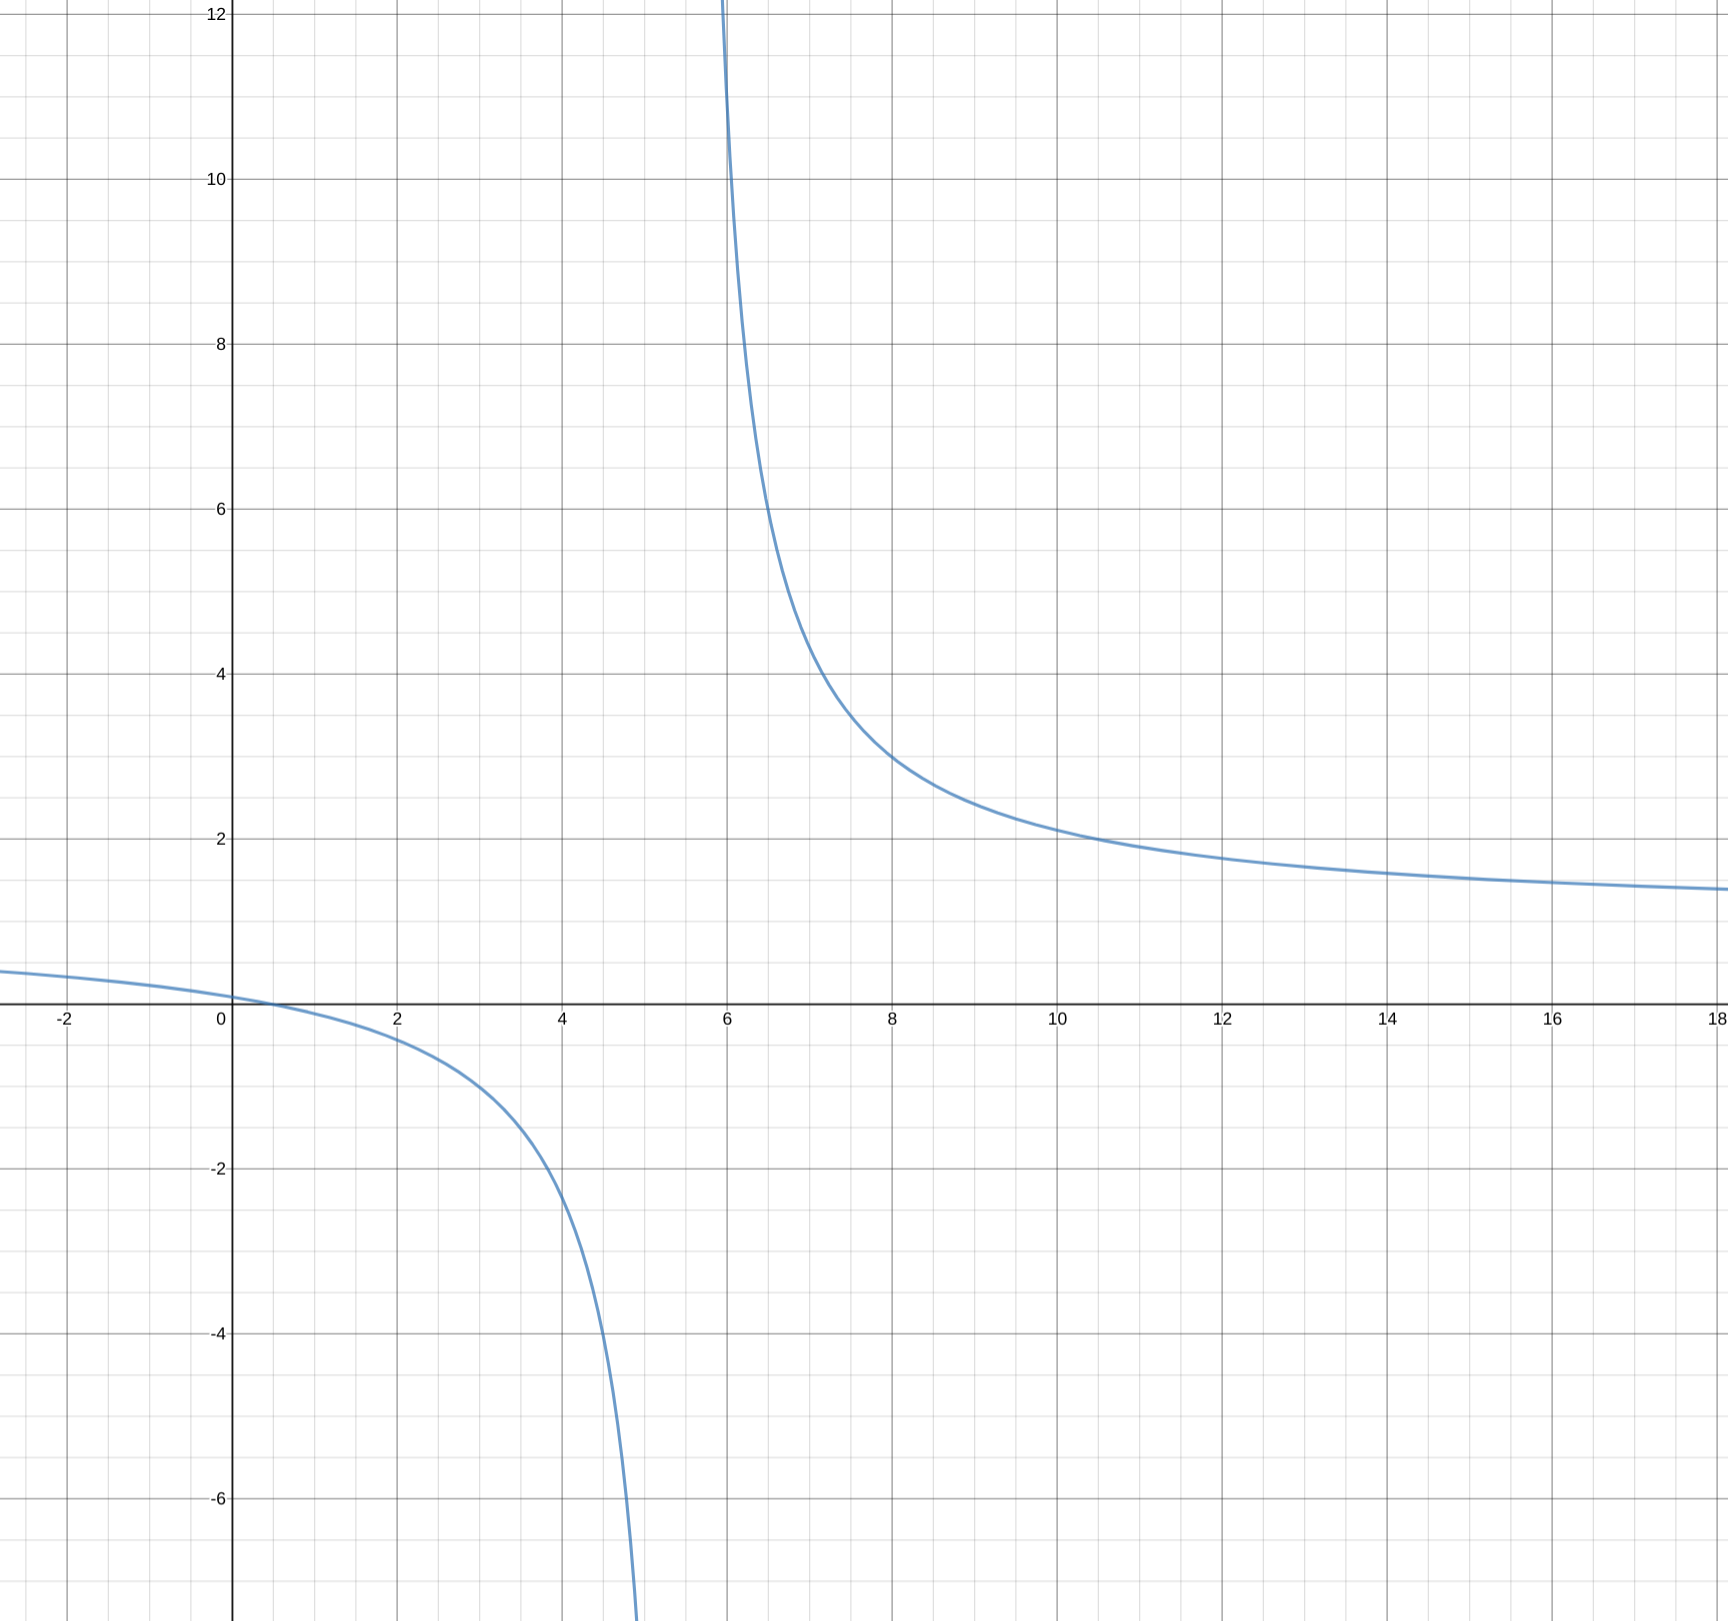
\includegraphics[scale=0.25]{invrad.png}
\item
Suppose I charge \$40 for each memebership to my Flight Data Monitoring (FDM) software anually, and our server is currently able to house 2,000 users comfortably. Lets say we have one of our stoarge disks fail, reducing this capacity to \$1,500 and we cannot afford a new one at the moment, causing me to now charge \$60 annually. Given the formula: $\epsilon_{a,b} = \frac{\% \Delta_p}{\% \Delta_q}$, we can substitute these values as such to determine our elasticity: \\
\begin{equation}
    \begin{split}
        \epsilon_{a,b} &= \frac{1500 - 2000}{1500 + 2000} * \frac{60 + 40}{60 - 40} \\
        \epsilon_{a,b} &= \frac{-500}{3500} * \frac{100}{20} \\
        \epsilon_{a,b} &= \frac{-1}{7} * 5 \\
        \epsilon_{a,b} &= \frac{-5}{7} \\
    \end{split}
\end{equation}
After taking the absoulte value of this result, we get $|\epsilon_{a,b}| = \frac{5}{7}$. This is a value less than $1$, which means that our price is relatively elasitc in this range. 

\item
    Context: Suppose I am an employee at a Company in New York that produces software to identify hazards for student pilots. The VP has just asked for a volunteer to evaluate a potential complement to our good (software). Cory and Landon are both co-workers who also happen to be software engineers, but not as well versed in economics as I am.\\
    \\
    \textbf{VP:} \say{So nobody wants to evaluate this new potential complement to our software?}\\
    \\
    \textbf{Me:} \say{I will. While I may just be a software engineer here, I took a few economics courses in college and gradaute school so I think I can find it out given my background.}\\
    \\
    \textbf{Cory:} \say{Well how do we know that you actually know what cross-price elasticity is? From what I remember, economics isn't a walk in the park, even for us computer scientists.}\\
    \\
    \textbf{Me:} \say{Good point, why don't I try to explain it to you guys, then we can refresh both of our memories!}\\
    \\
    \textbf{Landon:} \say{Well, I think I know what is meant by cross-price elasticity from my economics course in High School, but I'll hear you out}\\
    \\
    \textbf{Me:} \say{So, elasticity is basically just a quantified way to see how our product will interact with other potential complements and substitutes. What we want here is a good that is a very good complement, right!}\\
    \\
    \textbf{VP:} \say{Yes!}\\
    \\
    \textbf{Me:} \say{So, to make sure our product is a good complement to this product in Missouri, we would want the cross-price elasticity to be relatively elastic, implying that our software will not be substituted by theirs!}\\
    \\
    \textbf{Me:} \say{If we want to quantity this, the equation looks like (draws on chalkboard) $\epsilon_{a,b} = \frac{\% \Delta_p}{\% \Delta_q}$}\\
    \\
    \textbf{Cory:} \say{So, i'm assuming that that equation will give us numerical values that can tell us what the cross-price elasticity is?}\\
    \\
    \textbf{Me:} \say{Yes! So lets do an example. If for instance we keep selling our memebership at \$40 per year, and keep the same user base of about 10,000 users, but then decide to increase our price to \$45, we would want the absoulte value of the result of this equation to be greater than 1, and negative before we take the absoulte value. This would require our user base to increase as well. This would then imply that the cross-price elasticity is elastic and complementary, indicating that our product is a good complement to the one from our friends in Missouri. }\\
    \\
    \textbf{Landon:} \say{Well that would make sense because if they were a good substitute when we raised out price our user base wouldn't probably increase as well, right?}\\
    \\
    \textbf{VP:} \say{Right.}\\
    END.\\
\end{enumerate}
\end{document}
